\documentclass[a4paper]{article}
\usepackage[english, russian]{babel}
\usepackage[utf8]{inputenc}
\usepackage{graphicx}
\usepackage{fixltx2e}
\usepackage{hyperref}
\usepackage{multicol}
\usepackage[rightcaption]{sidecap}
\usepackage[top=1.5cm]{geometry}
\usepackage{tabularx}
\usepackage{array}
\usepackage{fancyhdr}
\usepackage{caption}
\usepackage{float}
\usepackage{amsmath}
\usepackage{upquote}

\pagestyle{fancy}
\fancyhead{}
\fancyfoot{}
\fancyfoot[R]{\thepage}

\begin{document}
\thispagestyle{empty}
\begin{center}
    \fontsize{12}{12}\selectfont{МИНИСТЕРСТВО НАУКИ И ВЫСШЕГО ОБРАЗОВАНИЯ РОССИЙСКОЙ ФЕДЕРАЦИИ

    \vspace{1em}
    ФЕДЕРАЛЬНОЕ ГОСУДАРСТВЕННОЕ АВТОНОМНОЕ ОБРАЗОВАТЕЛЬНОЕ УЧРЕЖДЕНИЕ ВЫСШЕГО ОБРАЗОВАНИЯ\\
    «Национальный исследовательский университет ИТМО»}

    \vspace{4em}
    \fontsize{16}{12}\selectfont{ФАКУЛЬТЕТ ПРОГРАММНОЙ ИНЖЕНЕРИИ И КОМПЬЮТЕРНОЙ ТЕХНИКИ}

    \vspace{4em}
    
    \fontsize{16}{12}\selectfont{\textbf{ЛАБОРАТОРНАЯ РАБОТА № 6}\\[1em]
по дисциплине «ИНФОРМАТИКА»}\\[1em]
    \fontsize{12}{12}\selectfont{Работа с системой компьютерной вёрстки \TeX}\\[1em]
    \fontsize{16}{12}\selectfont{Вариант № 71}
\end{center}

\vspace{10em}

\begin{flushright}
    \textbf{\textit{Выполнил:}} \\
    Студент группы P3107 \\
    Добрышкин Владимир Александрович\\
    \textbf{\textit{Преподаватель:}} \\
    Балакшин Павел Валерьевич \\
    (кандидат технических наук, доцент факультет ПИиКТ)
\end{flushright}
\vspace{13em}
\begin{center}
Санкт-Петербург, 2024
\end{center}
\setcounter{page}{22}
\begin{figure}[h]
    \centering
    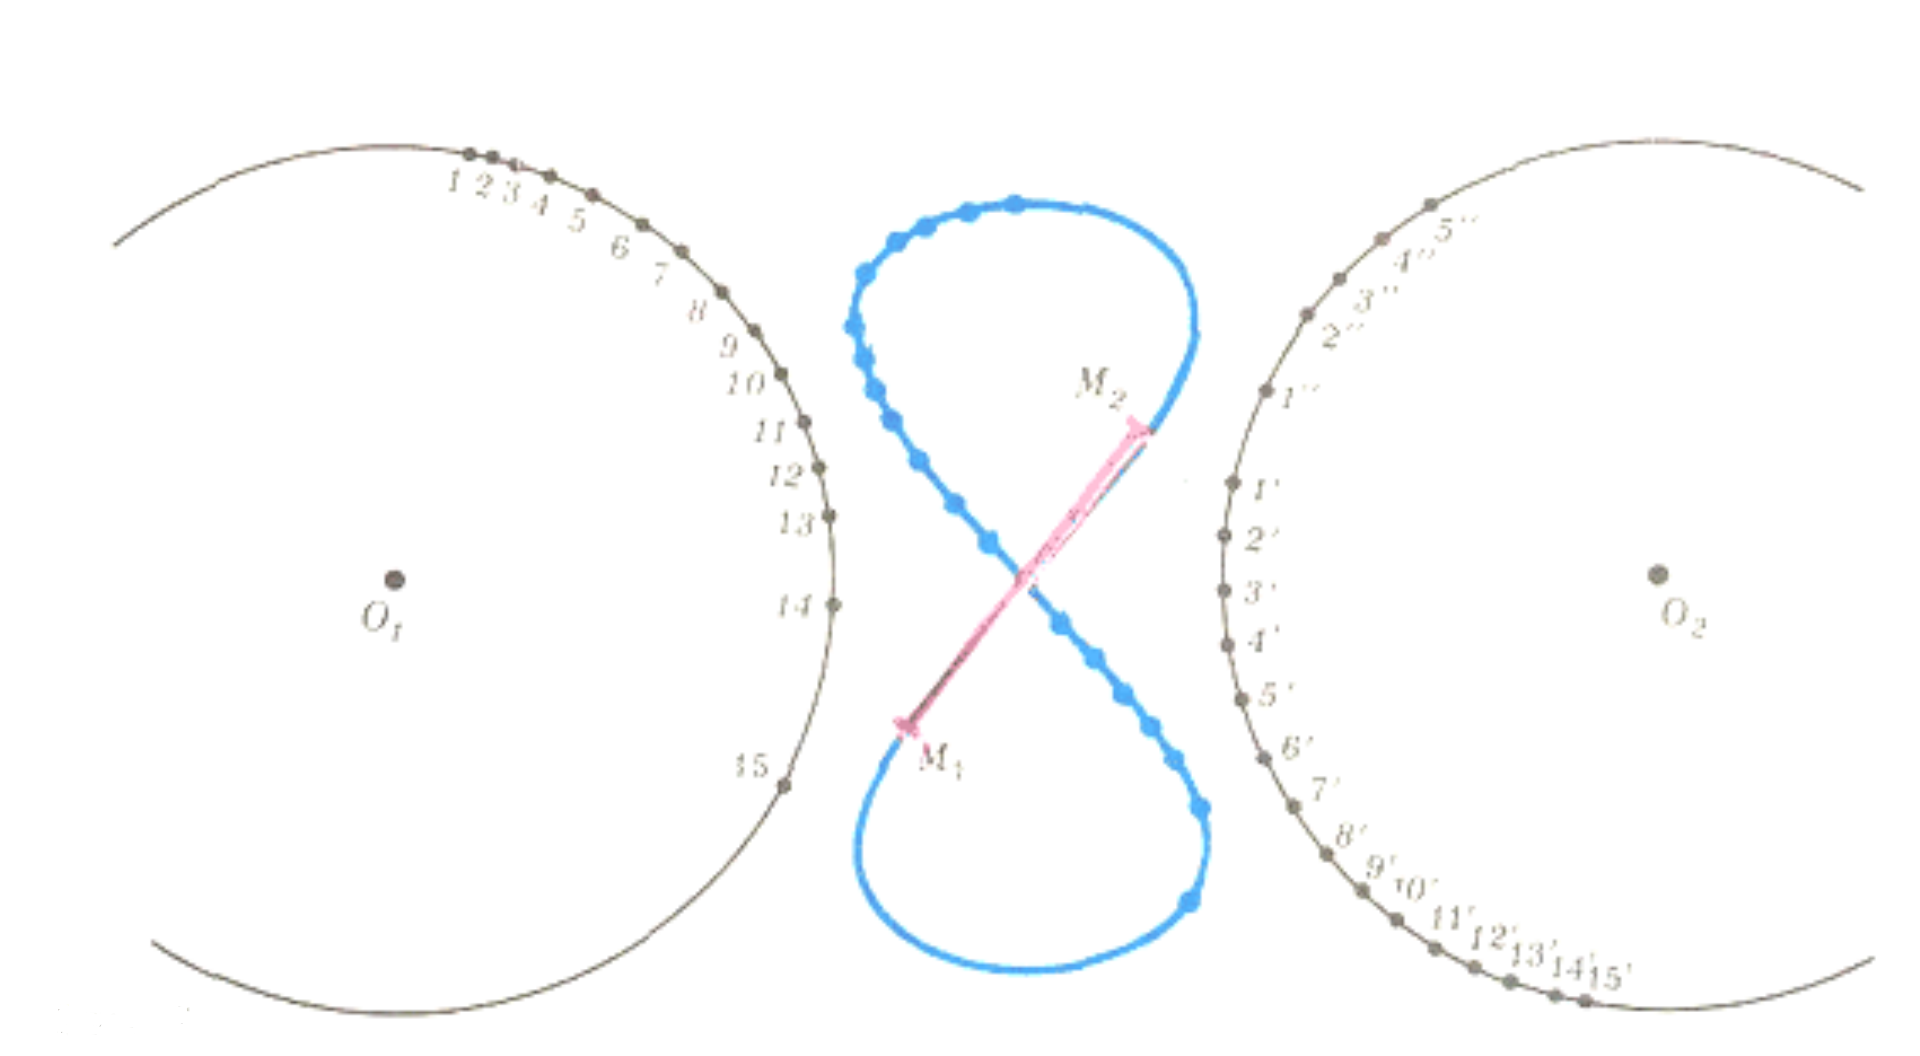
\includegraphics[width=0.85\textwidth]{scheme.png}
    \caption*{\raggedright \textbf{Рис. 7}}
    \label{fig:example}
\end{figure}
\vspace{-24.6pt} % Уменьшает расстояние между рисунком и текстом
\begin{multicols}{2}
    	% Вводите текст в первую колонку
    	\fontsize{12}{12}\selectfont{{Точки \(A_1\) и \(A_2\)могут перемещаться по окружностям радисуса \(R\) с центрами \(O_1\) и \(O_2\). Заметим, что наибольшее возможное значение расстояния \(|A_1 A_2|\) равно 2(\textit{l + R})(рис. 5,a), а наименьшее --- \(2(l - R\) (при \(l \leq R\)) или 0 (при \(l \geq R\)) (рис. 5, а, б). Отсюда следует, что для существования механизма Уатта необходимо, чтобы параметры \(d\), \(R\) и \(l\) удовлетворяли неравенствам  \[l - r \leq d \leq l + R.\]

	Мы будем говорить, что \textit{участок \(M_1M_2\) кривой отличается от отрезка прямой \(|M_1M_2|\) не более, чем на k \%}, если каждая точка \(M\) этого участка кривой удалена от отрезка \(M_1M_2\) на расстояние, не превосходящее \(a_0 = \frac{k}{100}|M_1M_2|\)(имеется в виду длина перпендикуляра из точки \(M\) на отрезок \(M_1M_2\); рис. 6).

	Теперь всё готово для того, чтобы сформулировать задание математического практикума.\medskip

\noindent{\textbf{Задание}}

\noindent{По параметрам \(d\),  \(R\) и \(l\) (см. таблицу) плоского шарнирного механизма Уатта:}

	a) начертите по точкам кривую Уатта, описываемую серединой шатуна;

	б) на построенной траектории при помощи линейки определите длину наибольшего участка кривой, отличающегося от отрезка прямой менее чем на 5 \%.\medskip

\noindent{\textbf{Образец}}

	\(d\) = 3; \(R\) = 4; \(l\) = 5 (рис. 5).}}

	
	\fontsize{9}{9}\selectfont{З а м е ч а н и е. Для самостоятельной работы возьмите один (или несколько) из наборов значенияяй \(d\),  \(R\) и \(l\) из таблицы. Положение точки \(М\) нужно находить при помощи циркуля и линейки: поставив одну ножку циркуля с раствором \(2d\) в некоторую точку \(Р\) окружности с центром в точке \(O_1\), радиуса \(R\), искать другой ножкой точку \(Q\) на второй окружности (с центром \(O_2\) радиуса \(R\)); середина отрезка \([PQ]\) определяется при помощи линейки. Число точек \(Р\), которое нужно взять для более или менее точного построения искомой траектории, равно 15; при вычерчивании кривой по построенным точкам нужно помнить о ее симметрии.

	После того как вы построите кривую, попробуйте ответить на несколько вопросов. 
	
$\textbf{1}^\circ$. На готовом чертеже покажите «полный цикл работы» механизма (т. е. то, как пе мещается шатун, когда его середина движет ся по кривой Уатта).

$\textbf{2}^\circ$. Сколько у данного механизма существует положений, из которых можно на чать движение более чем двумя способами?}
\end{multicols}
\vspace{-5pt} % Уменьшает расстояние между текстом и таблицей
{\begin{table}[H]
	\caption*{\raggedright \fontsize{9}{10}\selectfont{Т а б л и ц а}}
	\centering
    	\begin{tabularx}{\textwidth}{|>{\centering \arraybackslash}X|*{13}{>{\centering \arraybackslash}X|}}
        		\hline \rule{0cm}{0.8 cm} \centering
        		d&4&4&1&1&2&1&1&4&13&3&2&4 \\ \hline \rule{0cm}{0.8 cm} \centering
        		R&3&8&6&5&3&2&3&3&12&4&3&7 \\ \hline \rule{0cm}{0.8 cm} \centering
        		l&5&5&5&2&2&1&1&2&5&2&1&2 \\ \hline
    	\end{tabularx}
\end{table}
\newpage
\setcounter{page}{49}
\begin{multicols}{2}
\noindent{\textbf{Химический факультет}}

\textbf{1}. Решить уравнение \[|\cos x - \sin x| = 1 + \sin 2x\]

\textbf{2}. Решить неравенство \[\log_x(\frac{1}{7}) + \log_\frac{1}{7}{x} > 10|\log_\frac{1}{7}{x}|\]

\textbf{3}. Имеются два водных раствора № 1 и № 2 веществ \(А\) и \(Б\), различающиеся весовыми соотношениями веществ \(А\), \(Б\) и воды. В растворе № 1 вещества \(Б\) в 4 раза больше, чем вещества \(А\), а воды столько же, сколько вещества \(Б\). Смешав 3 \textit{кг} раствора № 1. 6 \textit{кг} раствора № 2 и добавив 1 \textit{кг} воды, получим новый раствор, в котором вещества \(А\) в 2 раза меньше, чем вещества \(Б\), и в 3 раза меньше, чем воды. Требуется определить весовое соотношение веществ \(А\), \(Б\) и воды в растворе № 2.

\textbf{4}. В равнобедренную трапецию вписана окружность с центром \(O_1\). Другая окружность с центром \(О_2\), расположенным вне вписанного круга, касается большего основания и боковой стороны трапеции. Обе окружности пересекаются и имеют общую хорду \(МN\). Известно, что \(\widehat{MO_1}N=60^\circ, \widehat{MO_2}N=120^\circ, |MN|=2\). Найти площадь трапеции.

\textbf{5}. Доказать, что уравнение \(2х - x^2 = \frac{2}{x}\) не имеет положительных решений.

\noindent{\textbf{Биологический факультет}}

\textbf{1}. Три экскаваторщика получили за дание вырыть три одинаковые канавы. Первый и второй экскаваторщики приступили к работе одновременно. Третий начал работу, когда второй вырыл пятую часть своей канавы, а закончил, когда первому оставалось вырыть четвертую часть своей канавы. Производительность второго экскаватора на 2 \(м/ч\) меньше, а производительность первого -- на \(4 м/ч\) меньше, чем производительность третьего экскаватора. Найти производительность третьего экскаватора. 

\textbf{2}. Решить неравенство \[2x^2 - |x|\log_3{78} + \log_3{26} < 1\] .

\textbf{3}. В треугольнике \(АВС\) проведена биссектриса \(BD\). Величины углов \(ADB\), \(BAD\), \(ABD\), \(АСВ\) в указанном порядке образуют арифметическую прогрессию. Найти длину высоты треугольника \(АВС\), опущенной из вершины \(С\), если известно, что \(|AB| = 1\). 

\textbf{4}. Найти все решения уравнения \[4 - 2\sin{x} - 3\cos{x} = 4\cos^2{(x - \frac{\pi}{3})} + \sqrt{3}(2 - \sin{x} - 2\cos{x}),\] которые одновременно являются и решениями уравнения \[2\sin{x} = \ctg{x} +3\tg^2{x} + \sqrt{3}\]

\textbf{5}. В кубе $A$\textit{В}$CDA'B'C'D'$, где [\textit{АА}\('], [BB'], [CC']\) и \([DD']\) -- параллельные ребра, плоскость \(\pi\) проходит через диагональ \(А'С\) грани куба и через середину ребра \(AD\). Найти расстояние от середины ребра \(АВ\) до плоскости \(\pi\), если длина ребра куба равна 3.
\end{multicols}
\end{document}